\documentclass[tikz]{standalone}
\usepackage{bm}
\usetikzlibrary{arrows}
\newcommand{\vect}{\bm}
\newcommand{\del}{\nabla}

\newcommand{\trans}[1]{{#1^\star}}
\newcommand{\surface}{h}
\newcommand{\shellcmd}[1]{\texttt{#1}}
\newcommand{\diffusioncoeff}{\mathcal{D}}
\newcommand{\exner}{\Pi}
\newcommand{\courant}{\mathrm{Co}}

\begin{document}
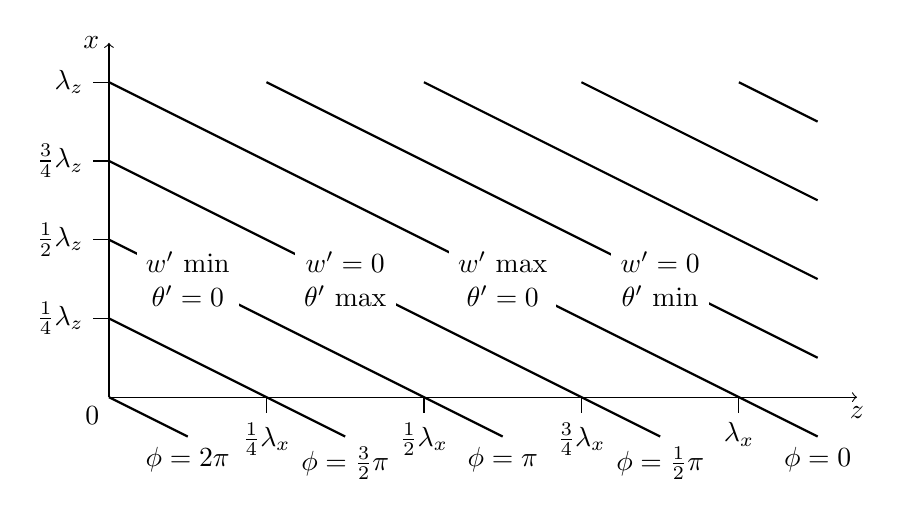
\begin{tikzpicture}[
  cpnt/.style={fill=gray},
  arr/.style={thick, ->},
]
\draw [->] (0,0) -- (0,4.5) node [at end, anchor=east] {$x$} node [at start, anchor=north east] {$0$};
\draw [->] (0,0) -- (9.5,0) node [at end, anchor=north] {$z$};

\draw [thick] (0,0) -- (1,-0.5) node [at end, anchor=north] {$\phi = 2 \pi$};
\draw [thick] (0,1) -- (3,-0.5) node [at end, anchor=north] {$\phi = \frac{3}{2} \pi$};
\draw [thick] (0,2) -- (5,-0.5) node [at end, anchor=north] {$\phi = \pi$};
\draw [thick] (0,3) -- (7,-0.5) node [at end, anchor=north] {$\phi = \frac{1}{2} \pi$};
\draw [thick] (0,4) -- (9,-0.5) node [at end, anchor=north] {$\phi = 0$};
\draw [thick] (2,4) -- (9,0.5);
\draw [thick] (4,4) -- (9,1.5);
\draw [thick] (6,4) -- (9,2.5);
\draw [thick] (8,4) -- (9,3.5);

\node [fill=white, align=center] at (1,1.5) {$w'$ min\\$\theta' = 0$};
\node [fill=white, align=center] at (3,1.5) {$w' = 0$\\$\theta'$ max};
\node [fill=white, align=center] at (5,1.5) {$w'$ max\\$\theta' = 0$};
\node [fill=white, align=center] at (7,1.5) {$w' = 0$\\$\theta'$ min};

\draw (0,1) -- (-0.2,1) node [at end, anchor=east] {$\frac{1}{4} \lambda_z$};
\draw (0,2) -- (-0.2,2) node [at end, anchor=east] {$\frac{1}{2} \lambda_z$};
\draw (0,3) -- (-0.2,3) node [at end, anchor=east] {$\frac{3}{4} \lambda_z$};
\draw (0,4) -- (-0.2,4) node [at end, anchor=east] {$\lambda_z$};

\draw (2,0) -- (2,-0.2) node [at end, anchor=north] {$\frac{1}{4} \lambda_x$};
\draw (4,0) -- (4,-0.2) node [at end, anchor=north] {$\frac{1}{2} \lambda_x$};
\draw (6,0) -- (6,-0.2) node [at end, anchor=north] {$\frac{3}{4} \lambda_x$};
\draw (8,0) -- (8,-0.2) node [at end, anchor=north] {$\lambda_x$};

\end{tikzpicture}
\end{document}
